\section{Datasets}\label{sec:datasets}

All six files are in FASTA format: a header line beginning with \texttt{>} followed by lines of sequence. The gene files carry their coordinates inside the reference genome in the header (for example \texttt{MN908947.3:21563-25384} for gene S), this gives an independent ground truth for the search algorithms.

Every file is read the same way. First, lines are stripped of whitespace and carriage returns (the DNA
files use Windows line endings), the header line is skipped, and the remaining symbols are
then uppercased. Any symbol outside $\{$A, C, G, T$\}$ for DNA, or outside the 20 amino-acid letters for
proteins, is counted and reported as unexpected. The check found no unexpected symbol in any of the six files
(Table~\ref{tab:datasets}).

\begin{table}[H]
    \centering
    \small
    \begin{tabular}{lrrccl}
\hline
file & length & symbols & most & least & unexpected \\
\hline
SARS-COV-2-MN908947.3.txt & 29903 & 4 & T & C & none \\
SARS-COV-2-MT106054.1.txt & 29882 & 4 & T & C & none \\
gen-ORF1AB.txt & 21290 & 4 & T & C & none \\
gen-S.txt & 3822 & 4 & T & G & none \\
gen-M.txt & 669 & 4 & T & G & none \\
seq-proteins.txt & 9701 & 20 & L & W & none \\
\hline
\end{tabular}
    \caption{Characterisation of the six files. Symbols counts the distinct expected symbols found.}
    \label{tab:datasets}
\end{table}

\begin{figure}[H]
    \centering
    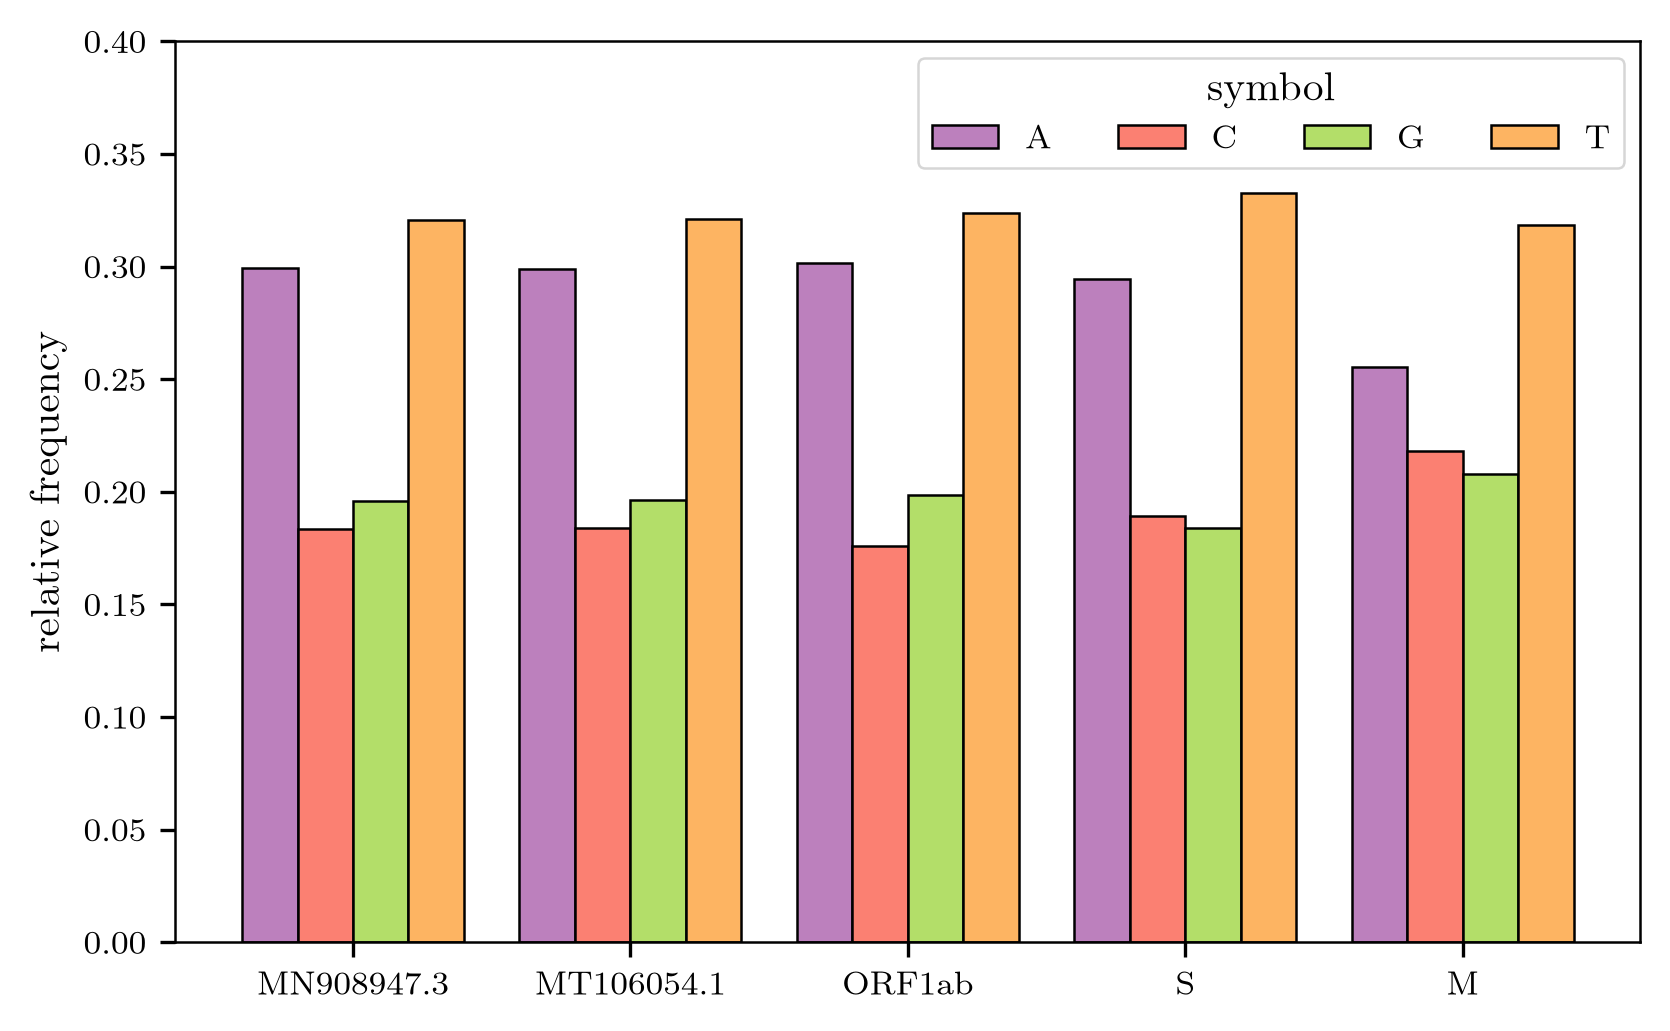
\includegraphics[width=0.6\textwidth]{fig_freq_dna}
    \caption{Relative nucleotide frequencies per DNA file.}
    \label{fig:freq}
\end{figure}

T is the most frequent base in every file. C is the least frequent in both genomes and in ORF1ab,
while in S and M the least frequent base is G. Gene M is the least skewed of the five DNA files. The
two genomes have practically identical composition (A 0.299, C 0.184, G 0.196, T 0.321 in both), a
first hint of how close they are before any alignment is computed. The amino-acid frequencies
(Figure~\ref{fig:freq_protein} in the appendix) are far from uniform: L is the most frequent and W
the least.
